%%%%%%%%%%%%%%%%%%%%%%%%%%%%%%%%%%%%%%%%%
% University Assignment Title Page 
% LaTeX Template
% Version 1.0 (27/12/12)
%
% This template has been downloaded from:
% http://www.LaTeXTemplates.com
%
% Original author:
% WikiBooks (http://en.wikibooks.org/wiki/LaTeX/Title_Creation)
%
% License:
% CC BY-NC-SA 3.0 (http://creativecommons.org/licenses/by-nc-sa/3.0/)
% 
% Instructions for using this template:
% This title page is capable of being compiled as is. This is not useful for 
% including it in another document. To do this, you have two options: 
%
% 1) Copy/paste everything between \begin{document} and \end{document} 
% starting at \begin{titlepage} and paste this into another LaTeX file where you 
% want your title page.
% OR
% 2) Remove everything outside the \begin{titlepage} and \end{titlepage} and 
% move this file to the same directory as the LaTeX file you wish to add it to. 
% Then add \input{./title_page_1.tex} to your LaTeX file where you want your
% title page.
%
%%%%%%%%%%%%%%%%%%%%%%%%%%%%%%%%%%%%%%%%%
%\title{Title page with logo}
%----------------------------------------------------------------------------------------
%	PACKAGES AND OTHER DOCUMENT CONFIGURATIONS
%----------------------------------------------------------------------------------------

\documentclass[12pt]{article}
\usepackage[english]{babel}
\usepackage[utf8x]{inputenc}
\usepackage{amsmath}
\usepackage{graphicx}
\usepackage[colorinlistoftodos]{todonotes}
\usepackage{hyperref}
\usepackage{listings}
\usepackage{appendix}
\usepackage{tabularx}
\usepackage{adjustbox}
\usepackage{multirow}
\usepackage{caption}
\usepackage{subcaption}
\usepackage{pgfplots}
\pgfplotsset{width=10cm,compat=1.9}
\usepgfplotslibrary{external}
\tikzexternalize


\begin{document}

\begin{titlepage}

\newcommand{\HRule}{\rule{\linewidth}{0.5mm}} % Defines a new command for the horizontal lines, change thickness here

\center % Center everything on the page
 
%----------------------------------------------------------------------------------------
%	HEADING SECTIONS
%----------------------------------------------------------------------------------------

\textsc{\LARGE University of Edinburgh}\\[1.5cm] % Name of your university/college
\textsc{\Large Programming Skills}\\[0.5cm] % Major heading such as course name
\textsc{\large Performance Testing Coursework}\\[0.5cm] % Minor heading such as course title

%----------------------------------------------------------------------------------------
%	TITLE SECTION
%----------------------------------------------------------------------------------------

\HRule \\[0.4cm]
{ \huge \bfseries Performance Report}\\[0.4cm] % Title of your document
\HRule \\[1.5cm]
 
%----------------------------------------------------------------------------------------
%	AUTHOR SECTION
%----------------------------------------------------------------------------------------



% If you don't want a supervisor, uncomment the two lines below and remove the section above
\Large \emph{Author:}\\
\textsc{Jack Frankland}\\[3cm] % Your name

%----------------------------------------------------------------------------------------
%	DATE SECTION
%----------------------------------------------------------------------------------------

{\large \today}\\[2cm] % Date, change the \today to a set date if you want to be precise

%----------------------------------------------------------------------------------------
%	LOGO SECTION
%----------------------------------------------------------------------------------------


\includegraphics[width=3cm, height=3cm]{logo.png}\\[3cm] % Include a department/university logo - this will require the graphicx package
 
%----------------------------------------------------------------------------------------

\vfill % Fill the rest of the page with whitespace

\end{titlepage}

\begin{abstract}
This report provides the results and analysis of various performance tests which were carried out on the 2D Predator-Prey model that was written for the first coursework. A range of different tests are used to evaluate the program and in each case the tests results are analyzed and interpreted. A conclusion is then reached about the overall quality of the program in terms of performance. 
\end{abstract}
\listoffigures
\listoftables
\tableofcontents

\section{Introduction}
\label{sec:introduction}
In order to provide a comprehensive performance analysis of the predator-prey simulation program we wrote, this report focuses on three different areas of testing. We begin by examining the effects of compiling the program under various compilers and their respective optimization flags on several different computers. This allows us to determine under which compiler and at which optimization level the program runs quickest. We then proceed to profile the program using a profiler tool. By identifying in which functions calls are the most computationally expensive we are able to identify the main overheads in our code, and in recognizing these overheads we can suggest possible optimizations that could result in faster code. Once we have finished investigating the performance of the code itself, we turn our attention to the performance of the code in terms of input and output. During its run the program outputs plain .ppm files at a frequency specified by the user; we investigate the performance effect of varying this frequency. Finally we test the code in terms of input by running it first with a range of landscapes with different land:water ratios, then with a range of landscapes of different sizes. This completes are performance testing, and based on our results we then make a general conclusion about the overall performance of the code.\\

Most of the performance tests in this document involve recording the runtime of the code for various independent variables. In order to get an accurate figure on the run time of the code in each test we initially planned to run the tests on the a single core on a Cirrus back end node. Because the traffic to Cirrus is fairly consistent, due to the fact is in constant use, this would have allowed us to make performance measurements we know are reconstructible, and hence could have compared run times with a good degree of confidence in their relative values. However, after some initial testing it was clear the code ran roughly 4-5 times faster on the cp-lab than it did on Cirrus. Further to this, we found that submitting several jobs to the Cirrus queue had the effect of slowing each job down by an amount proportional to the number of jobs submitted. The reason for this is not entirely clear; one possibility is that the different jobs were competing for memory on the front end node during output. This issue in particular made testing on Cirrus infeasible, since some run times were well over ten minutes, and the jobs needed to be submitted one at a time, the total runtime would have been too large to get any results. Instead we decided to use the cp-lab, since the run times were faster we were able to submit jobs individually and since the cp-lab is in use most of the time we can assume our results accurately represent a standard job runtime.

\section{Performance Tests and Analysis}
\label{sec:perf}

\subsection{Effects of Compiler Optimization Flags}
\label{subsec:opflags}
In this section we will investigate the performance effects of using different compilers with different optimization flags. To implement these tests we use a single $1000\times1000$ landscape given in figure \ref{fig:optlandscape} which consists of two large land masses separated by a river of water. This landscape was chosen since it is large enough and generic enough to provide results that could be scaled for any realistic landscape. The input parameters for all tests in this section were fixed as the values given in appendix \ref{ap:inputparameters}.
\begin{figure}
\centering
\frame{
\includegraphics[scale=0.2]{OpTestLandscape.png}}
\caption{Generic Test Landscape.}
\label{fig:optlandscape}
\end{figure}

We ran 6 tests for each compiler flag and calculated the mean and standard error using equations \ref{eqn:std} and \ref{eqn:stderr}. A complete set of measurements is given in \ref{ap:completedatasets}. For an explanation of what the various compiler optimization levels mean run any of \texttt{man clang++}, \texttt{man g++} or \texttt{man icpc} on a machine with the respective compiler installed and read the section on optimization flags.

\begin{table}[!h]
\begin{center}
\begin{adjustbox}{width=\textwidth,totalheight=\textheight,keepaspectratio}
\begin{tabular}{| c | c | c | c | c | c | c |}
\hline
\textbf{Compiler} & \multicolumn{6}{| c |}{\textbf{Run Time(s)}}  \\ 
\cline{2-7}
& \textbf{O0} & \textbf{O1} & \textbf{O2} & \textbf{O3} & \textbf{Ofast} & \textbf{Os} \\
\hline
gcc & $249.002 \pm 0.765$ & $181.647 \pm 0.571$ & $172.332 \pm 0.912$ & $174.978 \pm 0.777$ & $177.254 \pm
1.127$ & $190.362 \pm 0.496$\\ \hline
\end{tabular}
\end{adjustbox}
\end{center}
\caption{Run times for the $1000\times1000$ landscape in figure \ref{fig:optlandscape} running on the cp-lab.}
\label{table:optimizationcplab}
\end{table}

From these results it is clear that under the GNU g++ compiler the code runs fastest when compiled under the $\mathcal{O}2$ flag. This is slightly unexpected since one would expect the code to run fastest when compiled under the $\mathcal{O}3$ or $\mathcal{O}\text{fast}$ flags, however it is fairly common for different programs to run faster under different compiler flags due to the different optimisations the various compiler flags employ, and the content of the code itself.\\

We were interested in how well the program would perform under a completely different compiler, which is one of the reason we initially chose to use Cirrus. However, due to the fact the the cp-lab only has the GNU g++ compiler installed this meant using a different machine to compile the code. We chose to carry out these extra experiments on a Cirrus back end node and a Macbook to see how they would compare. Due to the long runtime for each test we were only able to carry out one test in each case and have not performed any statistical averages. 

\begin{table}[!h]
\begin{center}
\begin{adjustbox}{width=\textwidth,totalheight=\textheight,keepaspectratio}
\begin{tabular}{| c | c | c | c | c | c | c |}
\hline
\textbf{Compiler} & \multicolumn{6}{| c |}{\textbf{Run Time(s)}}  \\ 
\cline{2-7}
& \textbf{O0} & \textbf{O1} & \textbf{O2} & \textbf{O3} & \textbf{Ofast} & \textbf{Os} \\
\hline
clang & 529.025 & 457.535 & 395.897 & 415.884 & 383.270 & 399.656 \\ \hline
intel & 552.608 & 378.542 & 373.768 & 361.429 & 687.909 & 395.915 \\ \hline
\end{tabular}
\end{adjustbox}
\end{center}
\caption{Run times for the $1000\times1000$ landscape in figure \ref{fig:optlandscape} running on mid 2014 Macbook Pro with 2.8GHz Intel i5 processor with 8 GB 1600 MHz DDR3 memory.}
\label{table:optimizationmycomp}
\end{table}

\begin{table}[!h]
\begin{center}
\begin{adjustbox}{width=\textwidth,totalheight=\textheight,keepaspectratio}
\begin{tabular}{| c | c | c | c | c | c | c |}
\hline
\textbf{Compiler} & \multicolumn{6}{| c |}{\textbf{Run Time(s)}}  \\ 
\cline{2-7}
& \textbf{O0} & \textbf{O1} & \textbf{O2} & \textbf{O3} & \textbf{Ofast} & \textbf{Os} \\
\hline
gcc & 800.220 & 723.293 & 724.042 & 698.490	 & 698.005 & 734.928 \\ \hline
intel & 871.976 & 751.004 & 728.728  & 718.015  & 723.325  & 731.965 \\ \hline
\end{tabular}
\end{adjustbox}
\end{center}
\caption{Run times for the $1000\times1000$ landscape in figure \ref{fig:optlandscape} running on Cirrus back end node with 1 cpu.}
\label{table:optimizationcirrus}
\end{table}

From tables \ref{table:optimizationmycomp} and \ref{table:optimizationcirrus} we can see the Intel compiler produces an executable that runs fastest (relative to the machine it is compiled on) at the $\mathcal{O}3$ optimisation level. Since in the case of Cirrus the Intel compiler produces a program that runs faster than the GNU compiler, and on the Macbook the same Intel compiler produces a program that runs faster than the Clang compiler, this suggests that our program performs best when compiled under the Intel compiler. If the cp-lab had the Intel compiler suite installed it would be a good test to see how the run times of our program compared to the g++ results in table \ref{table:optimizationcplab} when compiled under the Intel icpc compiler. However, since the above results are not statistical averages it is difficult to make any definitive statement about any relative performance increase of code compiler under the Intel compiler; more results would need to be measured before any conclusions could be reached. The relative decrease in run time both in the case of the Macbook (compared to the Clang compiler) and Cirrus (compared to the GNU compiler), suggest there may be some performance bonus to compiling under the Intel compiler. 

\subsection{Main Sources of Overhead}
\label{subsec:overhead}
In order to identify the main sources of overhead in our program we used the GNU gprof tool. The code was compiled under the g++ compiler with optimisation level $\mathcal{O}$ (i.e. no optimizations) and without the debugging flags. This is because compiling with optimizations turned on can lead to inlining of functions, which in turn causes them to disappear from the profiling tables. However, since different compilers and different flags may inline different functions in different places, the profiling data would be specific to the compiler case, and not a general profile of the code. By compiling at $\mathcal{O}0$ level we can identify overheads that will be common to all compilers when there is no optimization. The input parameters and landscape are the same as in section \ref{subsec:opflags}. Since they are extensive and rather verbose we have included the first pages only since they contain the functions with the largest overheads.

\begin{figure}
\centering
\frame{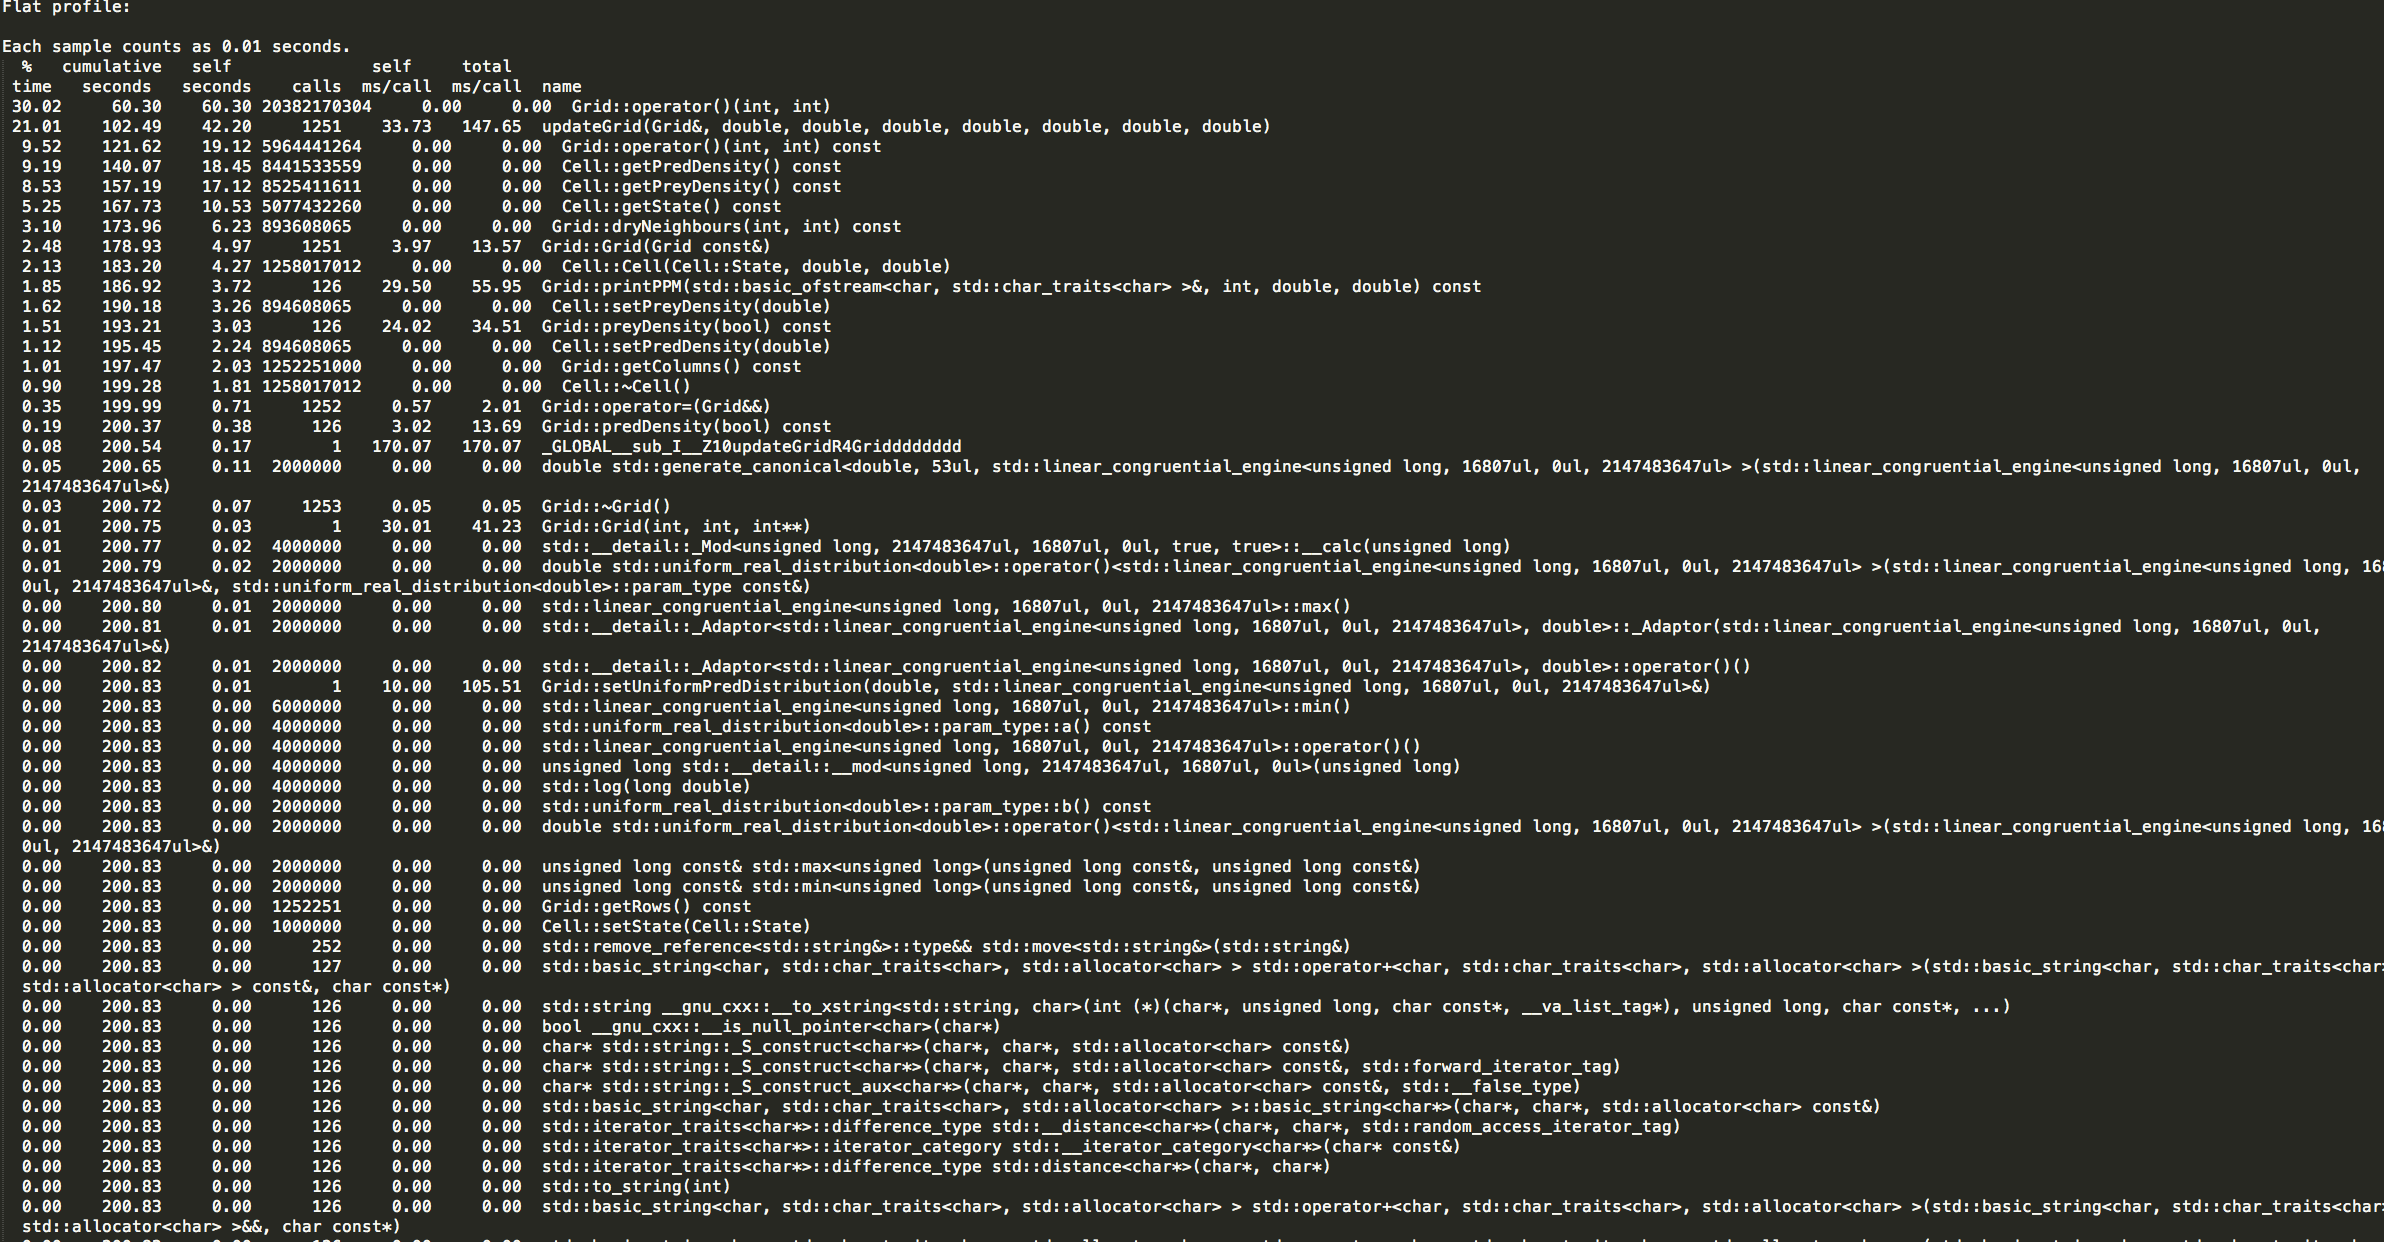
\includegraphics[scale=0.3]{Flat-Profile.png}}
\caption{Flat profile page 1. for GNU gprof profiler.}
\label{fig:flatp}
\end{figure}

\begin{figure}
\centering
\frame{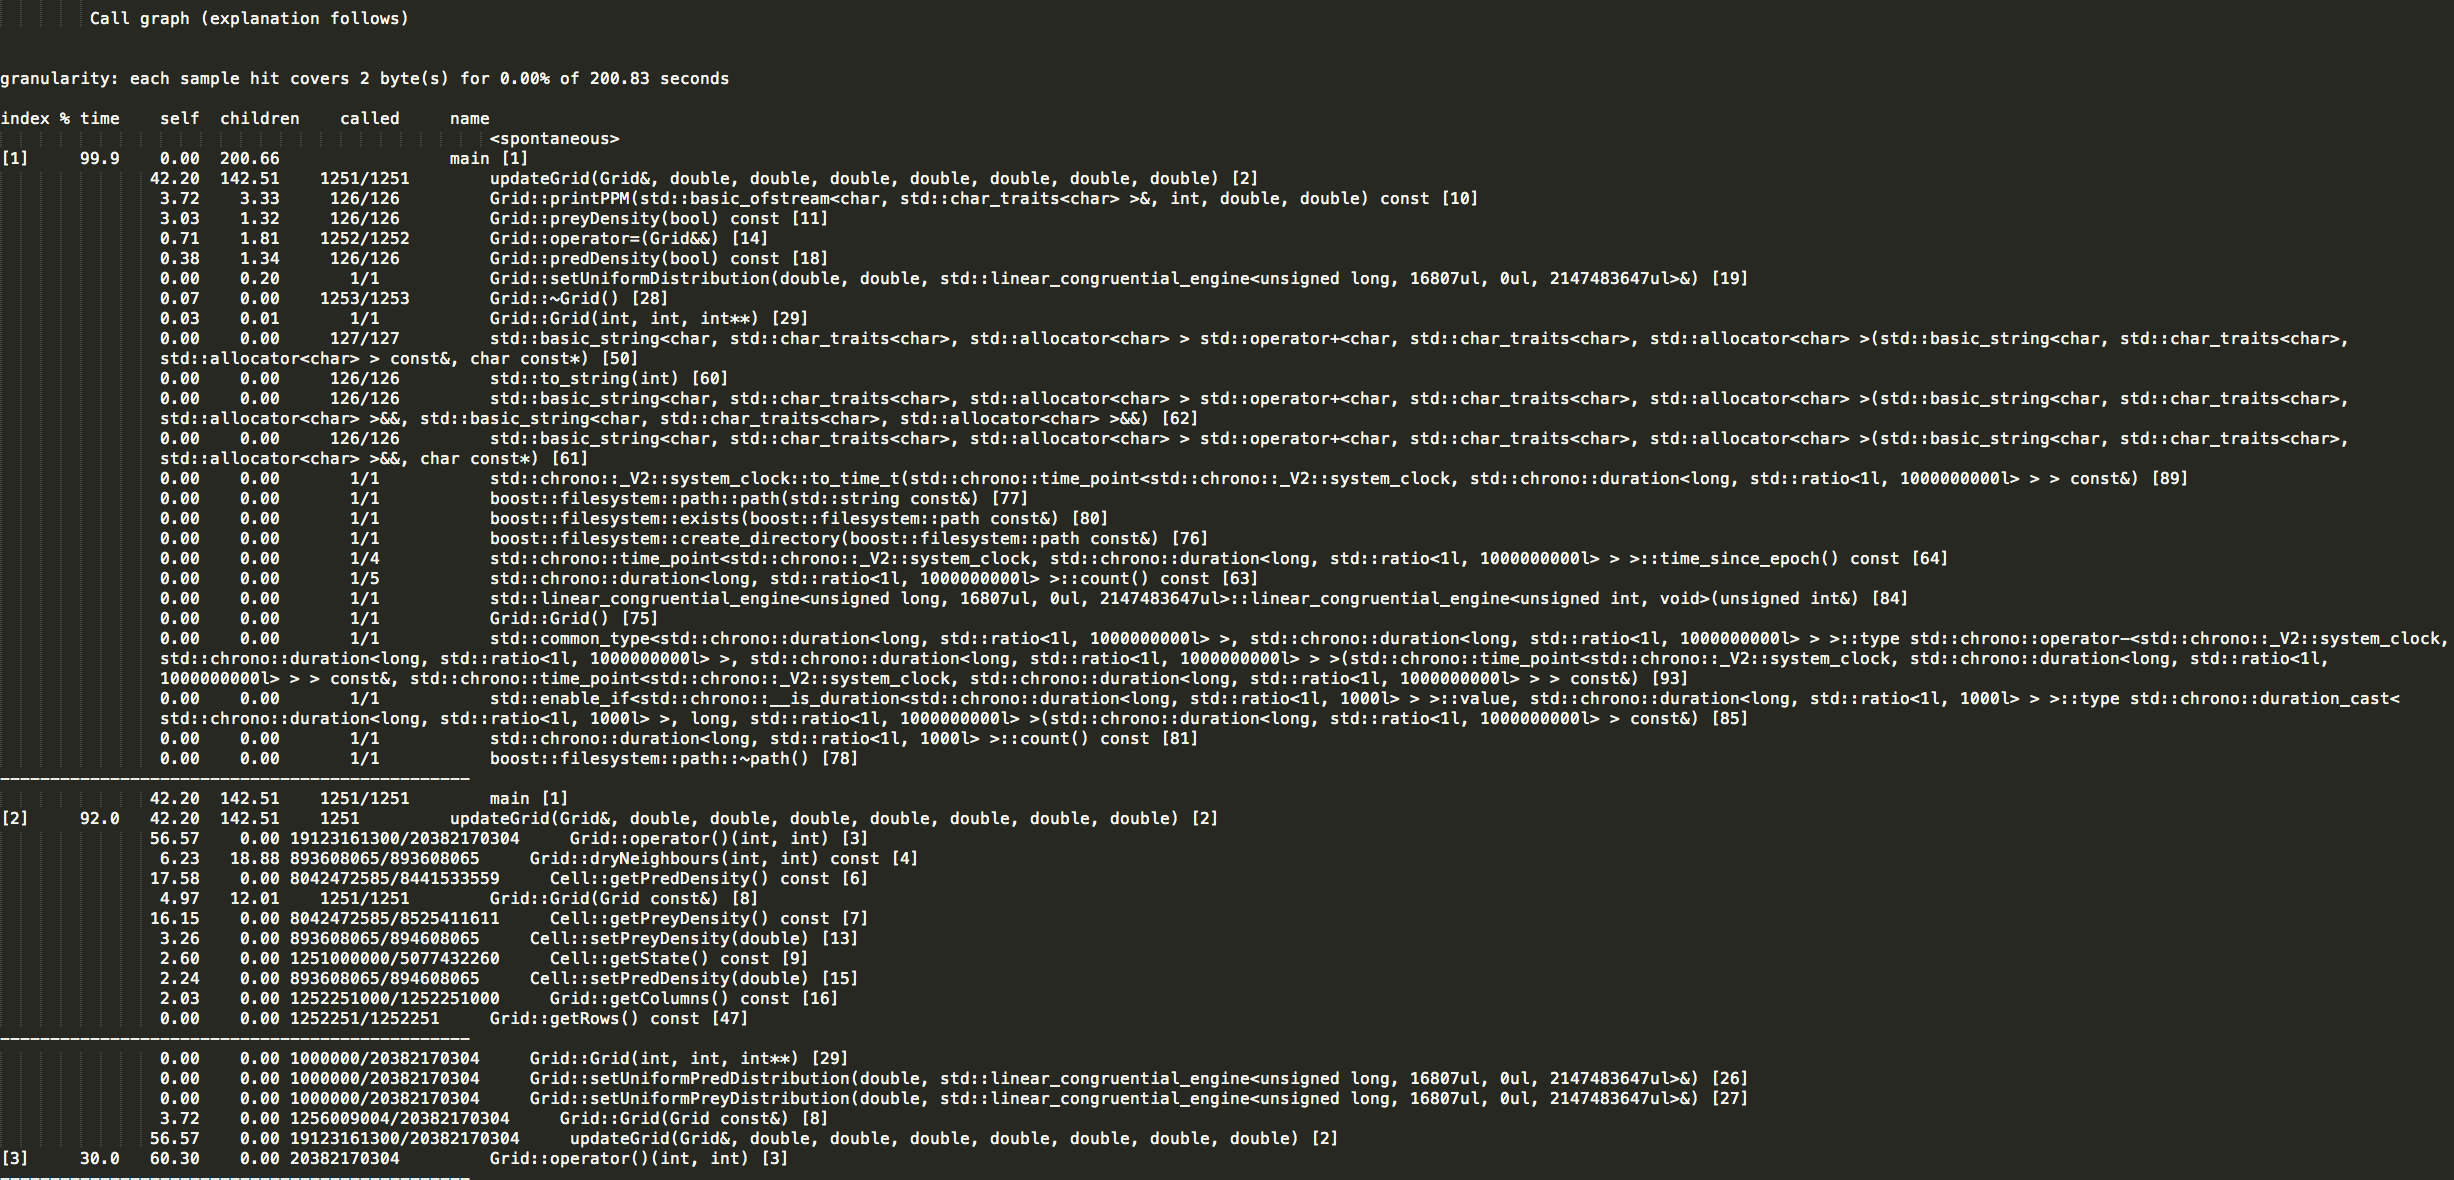
\includegraphics[scale=0.3]{Call-Graph-1.png}}
\caption{Call graph page 1. for GNU gprof profiler.}
\label{fig:callg}
\end{figure}

The \textit{flat profile} shows the total amount of time the program spent executing each function. From figure \ref{fig:flatp} we can see the program spent the most time executing the \texttt{operator()}. This is to be expected since the \texttt{operator()} function is used as a utility for accessing the landscape cells in the form \texttt{(i,j)}. Due to the fact that internally the landscape is implemented as a 1-D array this function was introduced to make working with the landscape simple and intuitive, and any time access to the landscape is required in the program, the \texttt{operator()} will have been used. One way to reduce the number of function calls to \texttt{operator()} would be to access the elements of the landscape directly in the code using the \texttt{operator[]} on the array of cells. This would make the code for the various Grid methods significantly harder to write and read since all instances of \texttt{operator(i,j)} would become \texttt{operator[[i + (rows + 1 - j) * (columns+2)]]}. An alternative would be to implement the landscape as a 2D array, then the access would be implemented via \texttt{operator[i][j]}, however it is likely the overhead of dynamically allocating a 2D array of a user defined type would outweigh the cost of the function we currently have. \\

The \textit{call graph} shows how much time was spent in each function and its children. Form this information we are able to identify functions that themselves do not use much time, but call other functions that use exceptional amounts of time. From figure \ref{fig:callg} line [2] we can see that $92\%$ of the time was spent in the function \texttt{updateGrid()} and its subroutines, which is to be expected since this is the function that evolves the landscape and apart from printing output, most the remaining functions called from the main method perform one off tasks such as setting up initial conditions. Of the function calls from within \texttt{updateGrid()} we can see that \texttt{operator()} clocks in the highest with $56.57\text{s}$ spent within it when it is called from \texttt{updateGrid()}. This supports our above analysis that the function \texttt{operator()} is a serious overhead. From [3] and [5] (not shown in figure \ref{fig:callg}) we can see that $39.5\%$ of the total time is spent in \texttt{operator()} or its constant equivalent. We can also see that it is the methods of the Grid class and the \texttt{updateGrid()} functions that call the \texttt{operator()}. Based on this analysis it would be a good idea to test giving these functions direct access to the grid cells through the \texttt{operator[]} instead of using the overloaded \texttt{operator()}. It may be that moving the functionality from \texttt{operator()} to \texttt{operator[]} means that the functions that call it inherit the overhead instead, however it is worth checking as a possible optimization. 

\subsection{Effects of Input/Output}
\label{subsec:input}

\subsection{Output Frequency}
\label{subsec:outfreq}
To begin the investigation into the effects of input we vary the number of time steps between the output of the plain .ppm files. The other input parameters are kept fixed at the same values in appendix \ref{ap:inputparameters}, however the number of steps between the output of the plain .ppm files is varied from 10 to 100 at intervals of 10 steps. The input landscape in figure \ref{fig:optlandscape} was used for the same reasons as in section \ref{subsec:opflags}. Since the program was shown to run fastest when compiled at the $\mathcal{O}2$ level in section \ref{subsec:opflags}, we have used that option here. 
\begin{figure}
\centering
\begin{tikzpicture}
\begin{axis}[
	xlabel= Number of time steps between output of plain .ppm file,
	ylabel= Run time (s),
    enlargelimits=true,
]
\addplot[color=red,mark=o,]
plot [error bars/.cd, y dir = both, y explicit]
table[x index=0, y index=1, y error index=2]{outputfrequencyforplot.txt};

\end{axis}
\end{tikzpicture}
\caption{Output frequency of plain .ppm vs run time (s)}
\label{fig:outfreqgraph}
\end{figure}

As in section \ref{subsec:opflags} we took six measurements for each output frequency and calculated the error using equations \ref{eqn:std} and \ref{eqn:stderr}. The error bars have been including in figure \ref{fig:outfreqgraph}, however they are very small. A complete set of measurements is given in \ref{ap:completedatasets}. It is clear from figure \ref{fig:outfreqgraph} that the runtime increases dramatically for higher frequencies, where as for lower frequencies the runtime increase is a lot slower. This relationship is perhaps made clearer in figure \ref{fig:outnumbgraph} where we have plotted the same run times against the total number of output files. The plot is clearly linear, which is what we would expect; the total runtime should be directly proportional to the number of files it outputs. The total number of output files can be calculated by dividing the total number of time steps by the frequency and then flooring the number.

\begin{figure}
\centering
\begin{tikzpicture}
\begin{axis}[
	xlabel= Total number plain .ppm output files,
	ylabel= Run time (s),
    enlargelimits=true,
]
\addplot[color=red,mark=o,]
plot [error bars/.cd, y dir = both, y explicit]
table[x index=0, y index=1, y error index=2]{outputnumberforplot.txt};

\end{axis}
\end{tikzpicture}
\caption{Number of output plain .ppm vs run time (s)}
\label{fig:outnumbgraph}
\end{figure}

\subsubsection{Landscape Water vs. Land}
\label{subsub:watervsland}
There are a myriad of possible ways to test the effects of varying the ratio of water to land in an input landscape. It is important to test the performance of the program using realistic input. For example, it would be possible to produce a landscape which was $50\%$ land $50\%$ water, where each pixel was alternatively water and land. Whilst this would be a valid input test landscape, it would not be a very good one, since it is so unrealistic it is unlikely anyone would ever try and model the evolution of a predator-prey system on a landscape of this sort. For these reasons we choose to test landscapes where land masses were always connected. In particular, to test the performance of the program under variation of the ratio of land to water in the input landscape we begun with the empty $1000 \times 1000$ landscape in \ref{fig:emptylandscape} (i.e. all water) and introduced strips of land of dimension $1000 \times 100$ ($10\%$ of the total landscape) e.g. figures \ref{fig:10landscape} and \ref{fig:20landscape}. By placing these strips underneath one another we produced eleven different landscapes each one having $10\%$ more land than the previous one, and eventually producing a landscape that was $100\%$ land i.e. figure \ref{fig:100landscape}. As in previous sections, we took six measurements at each land:water ratio and calculated errors using equations \ref{eqn:std} and \ref{eqn:stderr} and to shorten overall test times only output .ppm files every $100$ time steps. A complete set of measurements is given in \ref{ap:completedatasets}. Again, errors have been plotted in figure \ref{fig:watervslandgraph}, however they are very small. From section \ref{subsec:outfreq} we know that the runtime scales linearly with the number of output files produced. Thus in order to run quicker tests for the landscape size we ran with a low output frequency of 100 and assumed that for any other output frequency the result would scale linearly. All other input parameters are fixed as in appendix \ref{ap:inputparameters}.

\begin{figure} 
  \begin{subfigure}[b]{0.5\linewidth}
    \centering
    \frame{
\includegraphics[width=0.75\linewidth]{Fill0.png}}
    \caption{Initial landscape, $0\%$ land.} 
    \label{fig:emptylandscape} 
    \vspace{4ex}
  \end{subfigure}%% 
  \begin{subfigure}[b]{0.5\linewidth}
    \centering
    \frame{
\includegraphics[width=0.75\linewidth]{Fill100.png}} 
    \caption{2nd landscape with $10\%$ land.} 
    \label{fig:10landscape} 
    \vspace{4ex}
  \end{subfigure} 
  \begin{subfigure}[b]{0.5\linewidth}
    \centering
    \frame{
\includegraphics[width=0.75\linewidth]{Fill200.png}} 
    \caption{3rd landscape with $20\%$ land.} 
    \label{fig:20landscape} 
  \end{subfigure}%%
  \begin{subfigure}[b]{0.5\linewidth}
    \centering
    \frame{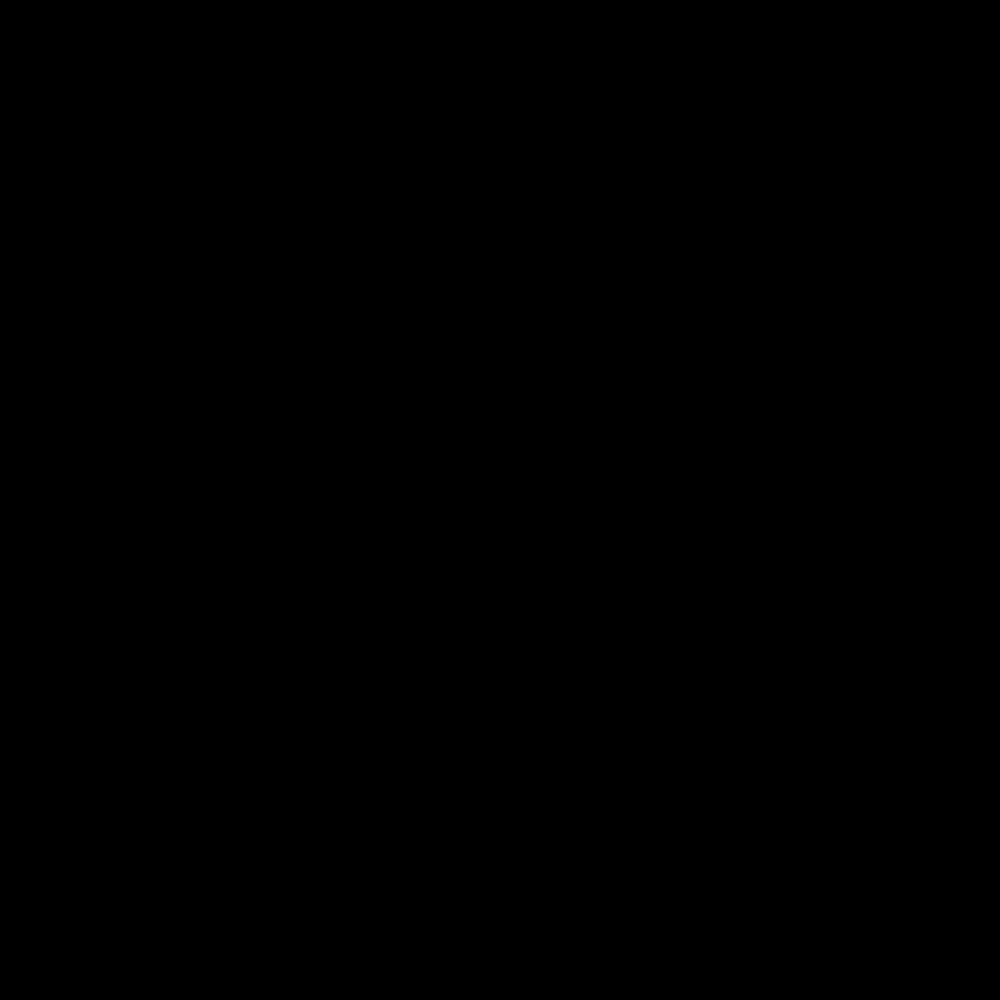
\includegraphics[width=0.75\linewidth]{Fill1000.png}} 
    \caption{Final landscape with $100\%$ land.} 
    \label{fig:100landscape} 
  \end{subfigure} 
  \caption{Examples of test landscapes for the water vs. land tests.}
  \label{fig:watervslandlandscape} 
\end{figure}


\begin{figure}
\centering
\begin{tikzpicture}
\begin{axis}[
	xlabel= \% of land in landscape,
	ylabel= Run time (s),
    enlargelimits=true,
]
\addplot[color=red,mark=o,]
plot [error bars/.cd, y dir = both, y explicit]
table[x index=0, y index=1, y error index=2]{watervslandforgraph.txt};



\end{axis}
\end{tikzpicture}
\caption{Water vs land runtime}
\label{fig:watervslandgraph}
\end{figure}

From figure \ref{fig:watervslandgraph} we can see that the run time scales linearly as the percentage of land in the landscape is increased. This is to be expected. Since the function \texttt{updateGrid()} first checks a cell in the landscape is water before updating it, and if it is water it ignores that cell; if we increase the number of land cells by say $10\%$ we increase the number of cells \texttt{updateGrid()} has to update on each call by $10\%$, and since each cell is roughly the same, we would expect the time taken to complete the update to increase linearly as a function of the number of cells needing to be updated, i.e. the percentage of the landscape that is land.

\subsubsection{Landscape Size}
\label{subsub:landscapesize}
To investigate the effects of varying landscape size for our program we scaled the square landscape of figure \ref{fig:optlandscape} using Gimp by increasing the width and height be equal amounts and recorded the time take to run in each case. For the same reasons as above, we ran with a low output frequency of $100$. As above we recorded six measurements at each landscape size and calculated standard error using equations \ref{eqn:std} and \ref{eqn:stderr}. A complete set of measurements is given in \ref{ap:completedatasets}. The results plotted in \ref{fig:landscapesizegraph} suggest a polynomial relationship between the size of the landscape and the run time of the form $\text{run time} = a (\text{landscape size}) ^k$. By taking the $\ln$ (natural log) of the data and plotting it in figure \ref{fig:loglandscapesizegraph} we can approximate the parameters $a$ and $k$ above by measuring the y-intercept and the gradient respectively. We can read off figure \ref{fig:loglandscapesizegraph}  $a \approx 2.718$ and $k \approx 2$, so we get the relationship $\text{run time} = 2.718(\text{landscape size}) ^2$ (for a complete explanation of this calculation see \ref{ap:parametercalculation}. The relationship $\text{run time} \propto (\text{landscape size}) ^2$ is to be expected, since the total area increases as the square of its sides for a square landscape, and we expect the run time to be proportional to the total area i.e. the number of squares in the landscape.
\begin{figure}
\centering
\begin{tikzpicture}
\begin{axis}[
	xlabel= Landscape size (square unit),
	ylabel= Run time (s),
    enlargelimits=true,
]
\addplot[color=red,mark=o,]
plot [error bars/.cd, y dir = both, y explicit]
table[x index=0, y index=1, y error index=2]{landscapesizeforplot.txt};
\end{axis}
\end{tikzpicture}
\caption{Size of square landscape vs run time (s)}
\label{fig:landscapesizegraph}
\end{figure}

\begin{figure}
\centering
\begin{tikzpicture}
\begin{axis}[
	xlabel= ln(landscape size),
	ylabel= ln(run time),
    enlargelimits=true,
]
\addplot[color=red,mark=o,]
plot [error bars/.cd, y dir = both, y explicit]
table[x index=0, y index=1, y error index=2]{loglandscapesizeforplot.txt};
\end{axis}
\end{tikzpicture}
\caption{Log plot of size of square landscape vs run time (s)}
\label{fig:loglandscapesizegraph}
\end{figure}

\section{Conclusion}
\label{sec:conclusion}

\begin{appendices}
\section{Complete Data Sets}
\label{ap:completedatasets}
These are the complete data sets for the performance experiments above, since tables \ref{table:optimizationmycomp} and \ref{table:optimizationcirrus} are complete, they are not repeated here:

\begin{table}[!htbp]
\centering
\label{tab:completeop}
\begin{tabular}{| c | c | c | c | c | c | c |}
\hline
{\textbf{Compiler} & \multicolumn{6}{| c |}{\textbf{Run Time(s)}}\\
\cline{2-7}
	& O0      & O1      & O2       & O3      & Ofast   & Os       \\
    \hline
    & 247.042 & 181.057 & 171.405  & 171.405 & 177.838 & 190.849 \\
    & 247.466 & 181.326 & 171.641  & 175.660 & 176.470 & 190.547 \\
gcc & 247.391 & 183.946 & 176.876  & 177.094 & 181.324 & 191.942 \\
    & 250.712 & 182.675 & 171.137  & 175.355 & 179.191 & 190.994 \\
    & 250.511 & 180.602 & 171.369  & 174.871 & 174.351 & 188.759 \\
    & 250.888 & 180.273 & 171.561  & 175.481 & 174.350 & 189.081\\ \hline
\end{tabular}
\caption{Complete data set for gcc optimisation tests on cp lab.}
\end{table}

\begin{table}[!htbp]
\centering
\label{tab:otsdata}
\begin{tabular}{| c | c | c | c | c | c | c |}
\hline
{\textbf{Number steps} & \multicolumn{6}{| c |}{\textbf{Run Time(s)}}\\
\hline
10  & 171.405 & 171.641 & 176.876 & 171.137 & 171.369 & 171.561\\
\hline
20  & 122.466 & 122.400 & 123.026 & 122.703 & 123.573 & 122.341\\
\hline
30  & 106.718 & 106.978 & 106.254 & 106.518 & 106.862 & 107.034\\
\hline
40  & 100.035 & 98.694  & 98.721  & 101.000 & 98.802  & 99.043\\
\hline
50  & 94.207  & 94.208  & 93.995  & 94.274  & 94.611  & 95.233\\
\hline
60  & 90.761  & 90.289  & 90.335  & 90.298  & 90.570  & 90.307\\
\hline
70  & 89.597  & 89.076  & 91.979  & 89.224  & 90.130  & 89662\\
\hline
80  & 88.188  & 87.924  & 86.422  & 87.013  & 86.457  & 86.422\\
\hline
90  & 84.877  & 84.799  & 84.838  & 84.877  & 84.945  & 85.100\\
\hline
100 & 84.151  & 84.138  & 84.095  & 84.392  & 84.051  & 84.146\\
\hline
\end{tabular}
\caption{Complete data set for varying number of steps between output of plain .ppm.}
\end{table}

\begin{table}[!htbp]
\centering
\label{tab:otsdata}
\begin{tabular}{| c | c | c | c | c | c | c |}
\hline
{\textbf{Landscape Size} & \multicolumn{6}{| c |}{\textbf{Run Time(s)}}\\
\hline
$200\times200$   & 3.372   & 3.409    & 3.711     & 3.366   & 3.3379   & 3.373\\
\hline
$400\times400$   & 14.431  & 13.768   & 14.803    & 14.029  & 13.848   & 13.881\\
\hline
$600\times600$   & 33.229  & 32.582   & 31.024    & 31.608  & 32.466   & 31.779\\
\hline
$800\times800$   & 55.585  & 56.726   & 55.295    & 55.303  & 54.997   & 55.709\\
\hline
$1000\times1000$ & 84.151  & 84.138   & 84.095    & 84.392  & 84.051   & 84.146\\
\hline
$1200\times1200$ & 126.580 & 131.212  & 125.095   & 127.586 & 124.953  & 128.426\\
\hline
$1400\times1400$ & 182.386 & 177.712  & 174.942   & 176.624 & 170.565  & 170.154\\
\hline
$1600\times1600$ & 222.399 & 220.579  & 221.788   & 222.024 & 222.322  & 226.443\\
\hline
$1800\times1800$ & 290.897 & 291.087  & 291.301   & 291.407 & 294.728  & 296.894\\
\hline
$2000\times2000$ & 359.388 & 360.973  & 360.214   & 367.307 & 356.216  & 344.524\\
\hline
\end{tabular}
\caption{Complete data set for varying landscape size.}
\end{table}

\begin{table}[!htbp]
\centering
\label{tab:wvldata}
\begin{tabular}{| c | c | c | c | c | c | c |}
\hline
{\textbf{\% Land} & \multicolumn{6}{| c |}{\textbf{Run Time(s)}}\\
\hline
$0\%$     & 26.948  & 28.551   & 27.910  & 29.626   & 28.183  & 27.691\\
\hline
$10\%$    & 35.243  & 35.205   & 35.047  & 35.283   & 35.396  & 35.147\\
\hline
$20\%$    & 43.009  & 43.200   & 43.356  & 42.989   & 43.240  & 43.471\\
\hline
$30\%$    & 51.306  & 51.047   & 50.895  & 50.968   & 51.930  & 51.395 \\
\hline
$40\%$    & 58.890  & 58.969   & 58.850  & 58.850   & 59.081  & 58.963\\
\hline
$50\%$    & 68.514  & 68.210   & 67.446  & 70.601   & 68.172  & 67.668\\
\hline
$60\%$    & 78.067  & 76.551   & 76.844  & 75.880   & 78.069  & 75.977\\
\hline
$70\%$    & 85.069  & 83.067   & 84.158  & 83.562   & 84.934  & 83.808\\
\hline
$80\%$    & 91.935  & 92.109   & 91.635  & 91.087   & 95.651  & 92.746\\
\hline
$90\%$    & 100.567 & 105.926  & 103.706 & 102.723  & 102.573 & 100.889\\
\hline
$100\%$   & 109.937 & 109.308  & 109.279 & 110.818  & 109.236 & 109.187\\
\hline
\end{tabular}
\caption{Complete data set for varying ratio of land to water.}
\end{table}


\section{Statistical Equations and Calculations}
\label{ap:stateqcalculations}
\subsection{Statistical Calculations}
\label{ap:statistics}
Our data sets were small due to the fact jobs had to be submitted individually to stop them slowing each other down. Because of this, we choose to use the \textbf{corrected sample standard deviation} given by:\tabularnewline
\begin{equation}\tabularnewline
\label{eqn:std}
s=\sqrt{\frac{1}{N-1}\sum^{N}_{i=1}(x_i-\bar{x})^2}
\end{equation}
which compensates for the bias in standard deviation which occurs for a small data set. The \textbf{standard error} was then estimated in the usual way using:
\begin{equation}
\label{eqn:stderr}
\sigma_x\approx\frac{s}{\sqrt{N}}
\end{equation}

\subsection{Parameter Calculation}
\label{ap:parametercalculation}
Given that we have some relationship between variables of the form:
\begin{equation}
y = ax^k
\end{equation}
then taking a general log of any base we get:
\begin{equation}
\log{y} = k\log{x} + \log{a}
\end{equation}
which is just the equation for a straight line between the variables $Y=\log{y}$ and $X=\log{x}$ with gradient k and y-intecept $C=\log{a}$. Hence if we can plot the logarithms of the values of $x$ and $y$ we can read of the exponent $k$ as the gradient and calculate $a = b^C$ where $b$ is the base of the logarithm.


\section{Input Parameters}
\label{ap:inputparameters}
These are the input parameters in the ``input\_parameters.txt'' used for all simulation tests, except in the case were the performance of the program was tested by varying the number of time steps between output of the plain .ppm file:
\begin{itemize}
	\item Birthrate of prey 0.08
	\item Predation rate at which predators eat prey 0.04
	\item Birth rate of predators per one prey eaten 0.02
	\item Predator mortality rate 0.06
	\item Diffusion rate of prey 0.2
	\item Diffusion rate of predators 0.2
	\item Size of time step 0.4
	\item Number of time steps between output of plain .ppm file 10
\end{itemize}

\end{appendices}
\end{document}